\documentclass[output=paper]{langsci/langscibook} 
\title{Number marking in Lopit, an Eastern Nilotic language} 
\author{%
Jonathan Moodie \affiliation{University of Melbourne}
}
% \chapterDOI{} %will be filled in at production


\abstract{
Nilotic and other Nilo-Saharan languages have rich number marking systems and it has been difficult to establish what rules might govern these systems \citep{Dimmendaal2000}. This paper addresses the question of how number is marked in Lopit and describes some possible rules for number marking. Lopit has a three-way system for number marking involving plurative, singulative and replacement marking. Lopit has a greater plural in addition to the normal plural. It also has a special form of number marking whereby the marked singular can be used to denote very large numbers. This form of number marking has not been observed in the literature and I call it the greater singular.
}

\maketitle
\begin{document}

\section{Introduction} \label{sec:moodie:1}

Lopit is an Eastern Nilotic language spoken by around 50,000 people living in the Eastern Equatoria province of South Sudan as well as by diaspora groups elsewhere in Africa and the world. It is part of the Lotuxo sub-group of the Lotuxo-Maa languages. Until recently, the Lopit language has received little descriptive attention. Some observations on Lopit were made by authors working on the related Otuho (Lotuko) language \citep{Muratori1938} and in comparative wordlist data collected by \citet{Driberg1932} and \citet{Vossen1982}. Lopit has only been the focus of linguistic description and documentation in more recent years. The language has six different dialects (Ngaboli, Dorik, Ngutira, Lomiaha, Lohutok and Lolongo), and data collected with speakers of a number of these has led to observations on aspects of Lopit phonetics and phonology \citep{Turner2001,Stirtz2014,Billington2014} and morphology and syntax \citep[e.g.][]{Laduetal2014}. Data presented in this paper are based on a corpus of elicited, storytelling and conversational materials collected with six Dorik speaking members of the Lopit community in Melbourne, Australia, transcribed and compiled using ELAN and Fieldworks. These speakers are aged between 30 and 55 and have migrated to Australia in the last 10 years.

The aim of this paper is to describe how number is marked in Lopit. There appears to be nothing in the literature about this subject apart from some singular and plural nouns in word lists given by \citet{Driberg1932} and \citet{Vossen1982}. I describe the different number marking patterns used, how these patterns are distinguished and what generalisations can be made about the selection of the number marking morpheme. In addition, I describe how Lopit uses two methods for expressing larger amounts than are normally described with plurals. I use the terms \textit{greater plural} and \textit{greater singular} to describe these methods. 

\section{An overview of number marking}\label{sec:moodie:2}

In many languages, a distinction can be made between countable and non-countable nouns. Non-countable nouns cannot be differentiated on the basis of number. They are called mass nouns. In Lopit, mass nouns are inherently either singular or plural.  The words for ‘milk’ and ‘water’ take plural agreement, whereas those for ‘air’, ‘grass’ and ‘flour’ take singular agreement. Examples are shown in \REF{ex:moodie:1} and \REF{ex:moodie:2}. In Lopit, relative clause pronouns inflect for the gender and number of the noun they modify.\footnote{Lopit is a tone language with high, low and falling tones. It has ATR distinctions which are not substantive in relation to number marking and are ignored in this paper. In general the Latin script is used as in English except that the sounds /x/, /ɲ/ and /ŋ/ are represented by {\textless}h{\textgreater}, {\textless}ny{\textgreater} and {\textless}ng{\textgreater} respectively.}

\ea\label{ex:moodie:1}
\gll r\`{e} h\`{u}n\'{a} l-\'{a}-r\'{a} h-\`{i}t\'{u}r\'{a} \\
milk \textsc{rel.f.pl} \textsc{sbo-3sg}-be \textsc{inf}-pour \\
\glt ‘sour milk’ (lit. ‘milk which has been poured’)
\z

\ea\label{ex:moodie:2}
\ea[]{\label{ex:moodie:2a}
\gll l\`{o}yy\'{a}m\`{i} n\`{a} l-\'{o}-n\'{o}k \\
air \textsc{rel.f.sg} \textsc{sbo-3sg}-be.hot \\
\glt ‘hot air’ (lit. ‘air which is hot’)}       

\ex[*]{\label{ex:moodie:2b}
\gll l\`{o}yy\'{a}m\`{i} h\`{u}n\'{a} l-\'{o}-n\'{o}k \\
air \textsc{rel.f.pl} \textsc{sbo-3sg}-be.hot \\}
\z
\z

Variation in the treatment of mass nouns also occurs in Turkana \citep[224]{Dimmendaal1983} and some Bantu languages \citep[173]{Corbett2000}. Dimmendaal ascribes these differences to the etymological origin of each particular term \citep[230]{Dimmendaal2000} rather than to any semantic conceptualization.

For countable nouns, Dimmendaal (\citeyear[224]{Dimmendaal1983}; \citeyear[214]{Dimmendaal2000}) has examined the patterns of number marking found in Nilo-Saharan languages and describes a tripartite system which is found in many of the languages in this family. This system is shown in \tabref{tab:moodie:1}, which has been adapted from \citet[224]{Dimmendaal1983} and \citet[156]{Corbett2000}. In Dimmendaal’s terminology, plurative marking is where the plural form has a morphological marker and the singular form is the unmarked base or root. Singulative marking is where the singular form has a morphological marker and the plural form is the unmarked base. Replacement marking is where both the singular and the plural forms have a morphological marker and the base is not specified for number and is not found as a word. The morphological markers are usually suffixes.\footnote{\citet[156]{Corbett2000} has also examined tripartite systems, largely using Nilo-Saharan examples. He uses a similar classification to Dimmendaal except that he uses the terms Type A, B and C for the plurative, singulative and replacement marking systems respectively. In this paper, I use Dimmendaal’s terms.}

\begin{table}
\begin{tabularx}{\textwidth}{lXXXXX}
\lsptoprule
\multicolumn{1}{c}{\textbf{System}} & \multicolumn{5}{c}{\textbf{Distinction}}\\
\midrule
plurative marking &  &  & base & \itshape versus & plural\\
singulative marking & singular & \itshape versus & base &  & \\
replacement marking & singular &  & \itshape versus &  & plural\\
\lspbottomrule
\end{tabularx}
\caption{The tripartite system of number marking}
\label{tab:moodie:1}
\end{table}

Lopit follows the tripartite system of singulative, plurative and replacement marking. Some examples are shown in \tabref{tab:moodie:2}. Note that there is a large range of segmental morphemes which can be used to mark number. This is discussed further in \sectref{sec:moodie:4}.

\begin{table}
\begin{tabularx}{\textwidth}{XXXX}
\lsptoprule

 \bfseries Marking System & \bfseries Singular & \bfseries Plural & \bfseries English\\ \midrule
\bfseries Singulative & {\itshape h\'{o}f\'{i}r-\'{i}}

{\itshape h\`{a}l\'{a}-t\'{i}}

\itshape \'{a}h\'{e}r-\'{i} & {\itshape h\'{o}f\`{i}r}

{\itshape h\`{a}l\`{a}}

\itshape \`{a}h\`{e}r & ‘feather’, ‘hair’

‘tooth’

‘star’\\
\bfseries Plurative & {\itshape b\'{e}r\`{e}t}

\itshape h\'{i}rr\'{i} & {\itshape b\`{e}r\'{e}t-\`{i}}

\itshape h\`{i}rr\`{i}-j\`{a} & ‘flag’

‘waterhole’\\
\bfseries Replacement & {\itshape h\'{u}ng-\'{u}}

\itshape f\`{a}\`{i}t-\^{i} & {\itshape h\`{u}ng-\`{a}}

\itshape f\`{a}\`{i}t-\^{o} & ‘knee’

‘ebony tree’\\
\lspbottomrule
\end{tabularx}
\caption{Tripartite system of number marking in Lopit}
\label{tab:moodie:2}
\end{table}

Some singular/plural relationships appear to involve irregular or suppletive forms. Some examples of these are shown in \tabref{tab:moodie:3}. There is some morphophonemic similarity between the singular and plural in all these examples. 

\begin{table}
\begin{tabularx}{\textwidth}{XXX}
\lsptoprule
 \bfseries Singular & \bfseries Plural & \bfseries English\\ \midrule
\itshape h\'{a}n\'{a} & \itshape h\`{a}ss & ‘hand’\\
\itshape m\'{a}n\'{a} & \itshape m\'{a}tt\'{a} & ‘farm’\\
\itshape h\'{i}t\'{e}ng & \itshape h\'{i}s\'{u}ng & ‘cow’\\
\itshape s\`{o}h\'{i}n\`{e} & \itshape s\'{a}ng & ‘thing’\\
\itshape w\'{o}r & \itshape w\'{o}nn\`{i} & ‘valley’\\
\lspbottomrule
\end{tabularx}
\caption{Irregular singular/plural forms}
\label{tab:moodie:3}
\end{table}

Another method of number inflection is tonal modification, although this has only been observed for a small number of nouns. No pattern has yet been discerned for the tonal alternations between singular and plural forms. Some examples are shown in \tabref{tab:moodie:4}.

\begin{table}
\begin{tabularx}{\textwidth}{XXX}
\lsptoprule

\mdseries \textbf{Singular} & \mdseries \textbf{Plural} & \mdseries \textbf{English}\\
\midrule
\itshape h\'{i}n\`{e} & \itshape h\`{i}n\`{e} & \mdseries ‘goat’\\
\itshape y\`{a}n\`{i} & \itshape y\'{a}n\'{i} & \mdseries ‘fruit, tree’\\
\itshape m\`{o}ny\`{e} & \itshape m\`{o}ny\^{e} & \mdseries ‘father’\\
\lspbottomrule
\end{tabularx}
\caption{Examples of tonal number inflection}
\label{tab:moodie:4}
\end{table}

I examined 446 Lopit nouns to determine the distribution of the various systems of number marking and to investigate potential rules. The frequency distribution of the different systems is shown in \tabref{tab:moodie:5}. The plurative marking system is the most common with 58\%, but the proportions of singulative and replacement marking patterns are both significant. 

\begin{table}
\begin{tabularx}{\textwidth}{XXX}
\lsptoprule

\mdseries \textbf{System } & \mdseries \textbf{Number} & \mdseries \textbf{Percent}\\ \midrule
Plurative & 257 & 58\\
Singulative & 85 & 19\\
Replacement & 79 & 18\\
Irregular \& tonal & 25 & 5\\
Total & 446 & 100\\
\lspbottomrule
\end{tabularx}
\caption{Distribution of number marking systems in Lopit}
\label{tab:moodie:5}
\end{table}

So far we have seen that Lopit has a variety of number marking morphemes and that most follow a tripartite marking system. We will now look at how the singulative and plurative marking systems in Lopit can be differentiated.

\section{The singulative and plurative distinction}\label{sec:moodie:3}

There is a semantic basis for the assignment of a lexeme to singulative versus plurative number marking pattern. The singulative pattern generally applies to those nominal lexemes which name referents which normally occur in groups or large numbers. In addition to the examples in \tabref{tab:moodie:2}, other nouns which are unmarked in the plural and take singulative marking include \textit{morro} ‘beans’, \textit{sana} ‘branches’ and \textit{sohot} ‘coconuts’. The singulative pattern is also used for nouns which are in pairs or finite sets (\textit{hafiela} ‘fingers’, \textit{iwwa} ‘wings’). This is common amongst Nilo-Saharan languages (\citealt[216]{Dimmendaal2000}; \citealt[119]{Creisselsetal2008}).

The distinction between singulative and plurative patterns can be related to the concept of individuation in number marking. \citet[217]{Corbett2000} points out that “the groups which we quantify with large numbers are the groups which are less individuated and conversely are more likely to be viewed as a unit”. Thus referents of the Lopit words \textit{aher}, ‘star’, \textit{balang}, ‘salt’ and \textit{hofir}, ‘hair’ are found in large numbers and are not easily differentiated into single items.

When they are individuated, singulative singulars can often have a specific meaning which refers to a separated item of the referent.  Some examples are shown in \tabref{tab:moodie:6}. 

\begin{table}
\begin{tabularx}{\textwidth}{XlXX}
\lsptoprule

\mdseries \textbf{Singular} & \mdseries \textbf{English} & \mdseries \textbf{Plural} & \mdseries \textbf{English}\\ \midrule
\itshape ngámá-rì & \mdseries ‘grain of sorghum’ & \itshape ngàmà & \mdseries ‘sorghum’\\
\itshape báláng-á & \mdseries ‘grain of salt’ & \itshape báláng & \mdseries ‘salt’\\
\itshape hófír-í & \mdseries ‘strand of hair’ & \itshape hófìr & \mdseries ‘hair’\\
\lspbottomrule
\end{tabularx}
\caption{Nouns that take the singulative patterns}
\label{tab:moodie:6}
\end{table}

The distinction between singulative and plurative has been examined in some detail by \citet{Grimm2012} for the Dagaare language (Gur: Niger-Congo).\footnote{ \citet{Grimm2012} uses the term \textit{marked singular} rather than \textit{singulative}.} He tested 1500 words in Dagaare and found the following \citep[50]{Grimm2012}:

\begin{enumerate}[label=\roman*.]
\item Nouns for higher-level (more salient) animals are more likely to be unmarked in the singular than nouns for insects. 
\item Nouns for trees are typically unmarked in the singular in comparison to nouns for vegetation which are typically unmarked in the plural. 
\item Nouns for tools are more likely to be unmarked in the singular than the converse. 
\item Nouns for body parts which inherently come in pairs or groups are more likely to be unmarked in the plural than not; while nouns for body parts which inherently come in single units are more likely to be unmarked in the singular.\footnote{There were a number of exceptions which related to some specific semantic aspects, borrowings and some derived forms.}
\end{enumerate}

I carried out a similar analysis on the set of 446 Lopit nouns and tested the categories of mammal, bird, reptile, insect, tree, vegetation and tool. The results are shown in \figref{fig:moodie:1}. The resulting trends were somewhat similar to those found by Grimm for the same categories. 

\begin{figure}
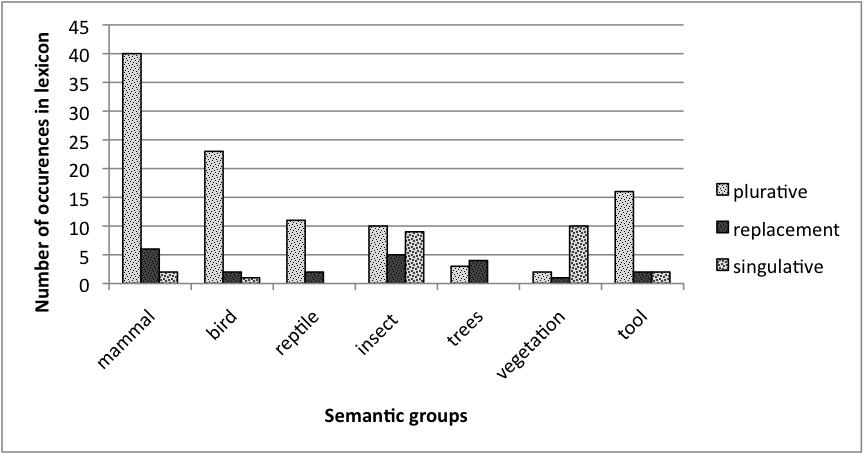
\includegraphics[width=\textwidth]{figures/moodie-fig-1.png}
\caption{Number marking across semantic domains}
\label{fig:moodie:1}
\end{figure}

For most semantic categories tested, the preferred number marking pattern was clear. However, it was not so clear for the insects and the data was examined in more detail. The examples of insects are listed in \tabref{tab:moodie:7}. Those insects which tend to be larger and more likely to be seen individually, such as butterflies, caterpillars and large wasps, take the plurative system. Conversely, those insects which are smaller and/or seen in large numbers such as mosquitoes, lice and flies have the singulative system. Whilst not conclusive, this data tends to support the role of individuation in determining the choice between singulative and plurative patterns for number markings.

\begin{table}
\begin{tabularx}{\textwidth}{llXllX}
\lsptoprule

\multicolumn{3}{c}{\textbf{Plurative}} & \multicolumn{3}{c}{\textbf{Singulative}}\\ \midrule
 \textbf{Singular} & \textbf{Plural} & \textbf{English} & \textbf{Singular} & \textbf{Plural} & \textbf{English}\\ \midrule
\itshape \'{i}f\`{o}r\'{i} & \itshape \`{i}f\`{o}r\'{i}-h\'{a} & ‘butterfly’ & \itshape h\`{i}l\'{o}f\`{i}r-\^{i} & \itshape h\`{i}l\`{o}f\`{i}r & ‘bee sp.’\\
\itshape l\`{o}m\'{o}l\`{o}r\'{u}k & \itshape l\`{o}m\'{o}l\`{o}r\`{u}h-\'{i} & ‘ant sp.’ & \itshape h\`{i}m\'{u}r\`{u}t-\'{i} & \itshape h\`{i}m\`{u}r\`{u}t & ‘mosquito’\\
\itshape h\`{u}t\`{e}l\`{e}k & \itshape h\`{u}t\`{e}l\'{e}h-\'{i} & ‘caterpillar’ & \itshape l\`{o}ng\'{o}r\`{o}m-\'{i} & \itshape l\`{o}ng\`{o}r\`{o}m & ‘termite’\\
\itshape \'{i}d\'{o}l\'{o} & \itshape \`{i}d\`{o}l\'{o}-h\'{o} & ‘locust’ & \itshape l\`{o}f\'{e}r-\`{i}t\'{i} & \itshape l\'{o}f\'{e}rr & ‘tick’\\
\itshape l\'{o}t\'{a}h\`{u}l\`{o}ng & \itshape l\`{o}t\`{a}h\`{u}l\'{o}ng-\'{i} & ‘wasp, large mud dauber’ & \itshape m\'{u}h\'{u}ny-\`{i} & \itshape m\'{u}h\'{u}ny & ‘ant, small black’\\
&  &  & \itshape \'{i}t\'{i}ng\'{i}l\`{i}y\`{e}-t\'{i} & \itshape \'{i}t\'{i}ng\'{i}l\`{i}y\`{e} & ‘ant, small brown’\\
&  &  & \itshape l\`{a}ki\`{e}-t\'{i} & \itshape l\`{a}ki\'{e} & ‘louse’\\
\lspbottomrule
\end{tabularx}
\caption{Plurative and singulative insect nouns}
\label{tab:moodie:7}
\end{table}

The number pattern for the terms for body parts was also investigated. The terms were grouped into those parts which are found singly (‘face’, ‘tongue’, ‘head’) and those which are found in pairs or sets (‘eyes’, ‘fingers’, ‘hands’). The results are shown in \figref{fig:moodie:2} and these also resemble the findings of Grimm.  That is, body parts which occur singly are more likely to have the plurative pattern and those parts found in pairs or sets are more likely to have the singulative pattern. 

\begin{figure}
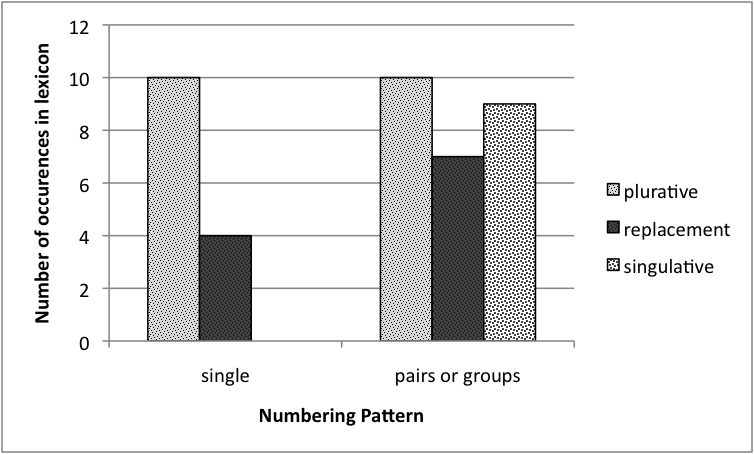
\includegraphics[width=\textwidth]{figures/moodie-fig-2.png}
\caption{The numbering patterns for body parts}
\label{fig:moodie:2}
\end{figure}

It is worth noting that there are a considerable number of examples of replacement marking in the body part data. Replacement marking is not found in Dagaare so this was not examined in Grimm’s (\citeyear{Grimm2012}) work. The proportion of the replacement system in some categories in Lopit is higher than for the singulative system.  In some groups, like ‘insects’ in \figref{fig:moodie:1} and  ‘pairs or groups’ in \figref{fig:moodie:2}, the proportion of replacement marking is quite high. From this data, it might be possible to infer that the proportion of replacement marking is higher for a particular semantic group when there are also high proportions of both singulative and plurative marking in the group. It could be that replacement marking is some kind of intermediate or derived pattern.  This is discussed further in \sectref{sec:moodie:4.3}.

One finding from this study does not appear to be reported by Dimmendaal or Grimm. This is the finding that some words are regarded as singulative by some speakers and plurative by others. Some examples are given in \tabref{tab:moodie:8}. For example, some speakers (AL, VH) consider the base of the concept of ‘rib’ or ‘ribs’ in Lopit (\textit{mari}) to be singulative in pattern with the singular marked by the suffix \textit{-ti}. A third speaker (DA) considers the base to be of the plurative pattern with the plural marked by the suffix \textit{-jin}. 

\begin{table}
\begin{tabularx}{\textwidth}{lllllllll}
\lsptoprule

\multicolumn{2}{c}{ \textbf{AL}} & \multicolumn{2}{c}{ \textbf{VH}} & \multicolumn{2}{c}{ \textbf{DA}} & \multicolumn{2}{c}{ \textbf{JL}} & \textbf{English}\\ \midrule
\textbf{SG} & \textbf{PL} & \textbf{SG} & \textbf{PL} & \textbf{SG} & \textbf{PL} & \textbf{SG} & 
 \textbf{PL} & \\ \midrule
\itshape m\`{a}r\'{i}-t\'{i} & \itshape m\^{a}r\`{i} & \itshape m\`{a}r\'{i}-t\'{i} & \itshape m\^{a}r\`{i} & \itshape m\`{a}r\'{i} & \itshape m\`{a}r\'{i}-j\'{i}n &  &  & ‘rib’\\
\itshape k\`{a}l\`{a}-\`{i} & \itshape k\`{a}l\'{a} & \itshape k\`{a}l\`{a}-\`{i} & \itshape k\`{a}l\'{a} & \itshape k\'{a}l & \itshape k\'{a}l-\`{i} &  &  & ‘side’\\
\itshape \`{i}-t\'{u}r\`{e}t & \itshape t\`{u}r\`{e}t &  & \itshape t\`{u}r\`{e}t / & {\itshape t\`{u}r\`{e}t } & {\itshape turet-i /}

& \itshape \`{i}-t\'{u}r\`{e}t & \itshape t\`{u}r\`{e}t & ‘twin’\\
&&& \itshape \`{i}-t\'{u}r\`{e}t && \itshape \`{i}-t\'{u}r\`{e}t-\'{i} & & \\
\lspbottomrule
\end{tabularx}
\caption{Examples of different speaker’s choice of singulative and plurative}
\label{tab:moodie:8}
\end{table}

This suggests that there is some kind of semantic boundary zone between those concepts which are more likely to take the singulative pattern and those that are more likely to take plurative pattern and that there might be variation between individuals on where this boundary sits. Ribs, sides and twins are found in sets with small numbers of members and are semantically more like individuated things. Thus they would be expected to be closer to the plurative marking. This suggests that, from a semantic perspective, these concepts might be viewed differently to concepts like hair and teeth.

\section{Regularity of number marking in Lopit}\label{sec:moodie:4}


\subsection{Introduction} \label{sec:moodie:4.1}


Many studies have commented on the complexity of number marking patterns in Nilo-Saharan languages and have pointed out that it is very difficult to predict the plural of a plurative pattern lexeme given the singular form of the lexeme (e.g.\ \citealt[4]{TuckerMpaayei1955}; \citealt[3]{HildersLawrance1957}). On the other hand, \citet[255]{Dimmendaal2000} states that Nilo-Saharan languages “have a finite system governed by rules” although he acknowledges that further research is required to understand these rules. 

This study has found that the forms of plurative, singulative and replacement marking in Lopit are very diverse. A large range of number suffixes was identified and this is common amongst Nilo-Saharan languages \citep[219]{Dimmendaal2000}. An attempt has been made to determine if there is a “finite system governed by rules”. The list of 446 nouns was examined and several patterns have been identified. These are shown in \tabref{tab:moodie:9}. 

\begin{table}
\begin{tabularx}{\textwidth}{lXXXXXX}
\lsptoprule

\multicolumn{2}{c}{ \textbf{Plurative}} & \multicolumn{2}{c}{ \textbf{Singulative}} & \multicolumn{3}{c}{ \textbf{Replacement}}\\ \midrule
 \textbf{Plural} & \textbf{Number} & \textbf{Singular} & \textbf{Number} & \textbf{Singular} & \textbf{Plural} & \textbf{Number}\\ \midrule
\itshape {}-i & 73 & \itshape {}-i & 30 & \itshape {}-ni & \itshape {}-k & 18\\
\itshape {}-hi & 5 & \itshape {}-ti & 34 & \itshape hi- & \itshape {}-i & 13\\
\itshape {}-a & 23 & \itshape {}-hi & 3 & {}-\textit{V}\textit{\textsubscript{1}}\textit{  } & \itshape {}-V\textsubscript{2} & 12\\
\itshape {}-ha & 32 & other suffixes & 18 & \multicolumn{2}{l}{other affixes} & 36\\
\itshape {}-o & 23 &  &  &  &  & \\
\itshape {}-ho & 16 &  &  &  &  & \\
\itshape {}-jin & 21 &  &  &  &  & \\
\itshape {}-(h,s,sh,c)in & 16 &  &  &  &  & \\
\hhline{~~~~---}
\itshape {}-Vn & 11 &  &  & Tonal &  & 9\\
other & 37 &  &  & Irregular &  & 16\\
suffixes & & & & & & \\
\lspbottomrule
\end{tabularx}
\caption{Patterns for singular and plural formation}
\label{tab:moodie:9}
\end{table}

The most common form (around 32\% of this sample) involves the suffix \textit{-i} or \textit{-Ci}. Note that this is found in both plural and singulative systems. Some examples are shown in \tabref{tab:moodie:10}.  

\begin{table}
\begin{tabularx}{\textwidth}{XXXXXX}
\lsptoprule

\multicolumn{3}{c}{ \textbf{Plurative}} & \multicolumn{3}{c}{ \textbf{Singulative}}\\ \midrule
 \textbf{Singular} & \textbf{Plural} & \textbf{English} & \textbf{Singular} & \textbf{Plural} & \textbf{English}\\ \midrule
\itshape t\`{i}\`{a}ng & \itshape t\`{i}\'{a}ng-\`{i} & ‘animal’ & \itshape c\`{e}ng-\^{i} & \itshape c\`{e}ng & ‘bird’\\
\itshape s\`{u}k\`{u}l & \itshape s\`{u}k\'{u}l-\'{i} & ‘school’ & \itshape f\'{o}f\'{o}ng-\`{i} & \itshape f\'{o}f\'{o}ng & ‘cactus’\\
\itshape g\'{a}l\'{a}m & \itshape g\'{a}l\`{a}m-\`{i} & ‘pen’ & \itshape s\`{u}k\'{a}r-\'{i} & \itshape s\`{u}k\'{a}r & ‘sugar’\\
\itshape b\`{u}k & \itshape b\`{u}h-\'{i} & ‘book’ & \itshape mu\'{a}r\'{a}h-\`{i} & \itshape mu\`{a}r\`{a}k & ‘horn’\\
\itshape s\`{a} & \itshape s\`{a}-t\'{i} & ‘hour’ & \itshape m\`{o}r\'{o}-t\'{i} & \itshape m\`{o}r\'{o} & ‘bean’\\
\itshape h\`{o} & \itshape h\`{o}-s\^{i} & ‘head’ &  &  & \\
\lspbottomrule
\end{tabularx}
\caption{Examples of number marking using \textit{-i} and \textit{{}-Ci}}
\label{tab:moodie:10}
\end{table}

A number of these examples are loan words (e.g.\ the words for ‘sugar’, ‘school’, ‘pen’ (Arabic) and ‘book’) and this suggests that these forms are productive.\footnote{ It is worth noting that, when the \textit{{}-i} suffix is added to a word ending in \textit{{}-k,} the consonant is modified to the velar fricative /x/ (represented here as {\textless}h{\textgreater}).} 

The suffix forms \textit{{}-a }and \textit{{}-o} also occur with both `singular' and `plural' meaning, as shown in \tabref{tab:moodie:11}. 

\begin{table}
\begin{tabularx}{\textwidth}{XlXXXX}
\lsptoprule

\multicolumn{3}{c}{ \textbf{Plural}} & \multicolumn{3}{c}{ \textbf{Singulative}}\\ \midrule
 \textbf{Singular} & \textbf{Plural} & \textbf{English} & \textbf{Singular} & \textbf{Plural} & \textbf{English}\\ \midrule
\itshape h\`{u}n\`{o}m & \itshape h\'{u}n\`{o}m-\`{o} & ‘cave’ & \itshape m\`{o}r\`{u}-\'{o} & \itshape m\'{o}r\'{u} & ‘stone’\\
\itshape h\`{u}r\'{o} & \itshape h\`{u}r\'{o}-h\'{o} & ‘goat kid’ & \itshape b\'{a}l\'{a}ng-\'{a} & \itshape b\`{a}l\`{a}ng & ‘salt’\\
\itshape h\'{o}mu\'{o}ng & \itshape h\`{o}mu\`{o}ng-\^{a} & ‘face’ &  &  & \\
\itshape h\'{a}r\'{i} & \itshape h\'{a}r\'{i}-y\`{a} & ‘river’ &  &  & \\
\lspbottomrule
\end{tabularx}
\caption{Examples of number marking with \textit{-a} and \textit{-o}} 
\label{tab:moodie:11}
\end{table}

For singulative marking, the suffix form appears to be more predictable.  In 75\% of the sample, the singular is marked with the suffix \textit{-i} after a stem-final consonant and with the suffix \textit{-ti} after a stem-final vowel. This is similar to the neighbouring Eastern Nilotic language, Lotuko, where \citet[7]{Arber1936} describes \textit{-i} as the “common form” for the singular suffix for singulative nouns 

\subsection{Suffixes for plurative number marking}\label{sec:moodie:4.2} 

One of the main things seen in the data in \tabref{tab:moodie:10} and \tabref{tab:moodie:11} is that it is not obvious how the choice between the \textit{{}-i}, \textit{-o}, and \textit{{}-a} suffixes is determined. \tabref{tab:moodie:12} shows the range of stem endings (i.e.\ the last two phonemes) that are associated with the various plural markers.

\begin{table}
\begin{tabularx}{\textwidth}{llX}
\lsptoprule

\multicolumn{1}{c}{\textbf{General}}& \multicolumn{1}{c}{\textbf{Suffix}} & \textbf{Last two phonemes on the stem}\\
\multicolumn{1}{c}{\textbf{suffix form}} & & \\ \midrule
\itshape {}-(C)i & \itshape {}-i & {}-ak, -am, -an,-ang, -at, -eng, -ek, -el, -er, -et, -ing, -ir, -it, -of, -ol, -om, -ong, -or,  {}-os, -ra, -re, -ru, -uk, -ul, -um, -uny, -ur, -ut, -wa\\
\hhline{~--} & \itshape {}-hi & {}-du, -fi, -f\textipa{\super w}o, -fa\\
\hhline{~--} & \itshape {}-ni & {}-ra\\
\hhline{~--} & \itshape {}-si & {}-bu, ho,\\
\hhline{~--} & \itshape {}-ti & sa, -ju, -iu, -me, -re, -ri, -ro, -ye, \\ \midrule
\itshape {}-(C)a & \itshape {}-a & {}-ak, -al, -ar, -ang, -bu, -ef, -en, -er, -ir,-ok, -ol, -ong, -ni\\
\hhline{~--} & \itshape {}-ha & {}-ga, -gu, -ia, -ja, -la, -le, -ne, -ra, -re, -ri, -ti, -tu\\
\hhline{~--} & \itshape {}-ja & {}-ri, -tu\\
\hhline{~--} & \itshape {}-na & {}-ge, -ha\\
\hhline{~--} & \itshape {}-ta & {}-he, -ri\\
\hhline{~--} & \itshape {}-ya & {}-me, -ni, -ri, -te\\ \midrule
\itshape {}-(C)o & \itshape {}-o & {}-ing, -ol, -om, -ong, -ony, -ri, -ru, -ti\\
\hhline{~--} & \itshape {}-ho & {}-lo, -me, -mu, -ri, -ro, -ti, -wo\\
\hhline{~--} & \itshape {}-jo & {}-ti\\
\hhline{~--} & \itshape {}-so & {}-he\\
\hhline{~--} & \itshape {}-yo & {}-mi, -ni, -ri\\
\lspbottomrule
\end{tabularx}
\caption{Plural suffixes with the stems to which they attach}
\label{tab:moodie:12}
\end{table}

A large range of final vowel, consonant, and vowel/consonant combination can be found with each of the three suffix types. This shows that suffix choice cannot be predicted based on how the noun stem ends. However, there were occasional tendencies for words with similar structures to pattern together, so this was examined further.

To explore what suffix choices might be regularized, three consultants were tested on their intuitions about the plural marking of loan words from English and Arabic and of nonce words.\footnote{ A nonce word is one which has been made up for testing purposes. Since consonant clusters are not normally found in Lopit words, the testing was based on CV(CV)(C) words. Sometimes, consultants also gave Arabic plurals e.g.\ \textit{kabaya}, \textit{kabaya-t} and these have been ignored.} A smaller sample of 66 words was used and several patterns were identified. The syllable structure of the stem appears to play a role. The results are shown in \tabref{tab:moodie:13} together with some examples.

\begin{table}
\begin{tabularx}{\textwidth}{XllXlXX}
\lsptoprule

\small \textbf{Stem} & \small \textbf{Singular} & \small \textbf{Plural} & \small \textbf{English} & \small \textbf{Suffix} & \small \textbf{No.\ of}  & \small \textbf{No.\ of} \\ [-.15em]
\small \textbf{structure} & & & & & \small \textbf{words with this stem structure} & \small \textbf{words with this suffix} \\ \midrule
\mdseries consonant final & \itshape batik & \itshape batih-i & \mdseries `water\-melon' & \itshape {}-i & \mdseries 40 & \mdseries 39\\
& \itshape gamis & \itshape gamis-i & \mdseries ‘shirt’ &  &  & \\
& \itshape telifision & \itshape telifision-i & \mdseries ‘television’ &  &  & \\
\mdseries CV & \itshape ka & \itshape ka-si & \mdseries ‘car’ & \itshape {}-si & \mdseries 5 & \mdseries 3\\
\mdseries CVCV & \itshape leta & \itshape leta-sin & \mdseries ‘letter’ & {\itshape {}-sin,}
 & \mdseries 11 & \mdseries 9\\
& \itshape tivi & \itshape tivi-sin & \mdseries ‘TV’ &  \itshape {}-jin &  & \\
\mdseries CVCVCV & \itshape kubaya & \itshape kubaya-ha & \mdseries ‘cup’ & \itshape {}-ha & \mdseries 10 & \mdseries 5\\
& \itshape natana & \itshape natana-ha & \mdseries nonce word &  &  & \\
& \itshape teroli & \itshape teroli-ho & \mdseries ‘trolley’ & \itshape {}-ho &  & \mdseries 3\\
& \itshape pomodi & \itshape pomodi-ho & \mdseries nonce word &  &  & \\
\lspbottomrule
\end{tabularx}
\caption{Results from the study with loan and nonce words}
\label{tab:moodie:13}
\end{table}

The tests with borrowed and nonce words show patterns which are also present to some extent in the previous lexical data, but with much more irregularity. This suggests that there are some preferences governing choice of number-marking morpheme, allowing the system to be productive, but that historical or other processes may have obscured parts of this system in the Lopit lexicon. On the basis of the tests, the following generalisations for plural formation are provisionally proposed.\footnote{I assume that there is a single morpheme (provisionally called -\textit{sin}) which has variable pronunciations which may in part be lexically specified and may also differ depending on the individual. These include -\textit{shin,-sin, -cin }and \textit{{}-jin}.}

\ea\label{ex:moodie:3} If the noun ends in a consonant, the plural suffix is \textit{-i}

If the noun has the form CV, the plural suffix is \textit{-si} 

If the noun has the form CVCV, the plural suffix is \textit{-sin} 

If the noun has the form CVCVCV and at least one V is\textit{ o}, the plural suffix is \textit{-ho} 

If the noun has the form CVCVCV and at least one V is \textit{a}, the plural suffix is \textit{-ha} 
\z

Variation in plural formation in Turkana is similarly related to word structure. \citet[235]{Dimmendaal2000} gives examples of the plurative suffix \textit{{}-a}, which is found after CVCVC roots, and the suffix \textit{{}-in}, which is found after CVC roots. 

It is also worth noting that there is some variation between speakers. Some of this is may be related to different locations within the same dialect area. However, there is also some variation with the same speaker such as alternating between common suffixes like \textit{-ho} and \textit{-sin}. This was also observed by \citet[76]{Unseth1988} in his study of the Nilo-Saharan Surmic language, Majang. He commented that “A certain amount of variation for marking number on some nouns is noticeable, even by one speaker” and that “Generally, the variation consisted of alternate suffixes”. This variation is not surprising given the complexity of the number-marking systems. In addition, alternating some of the common suffixes for plurative nouns is unlikely to cause much ambiguity.

\subsection{Affix forms for replacement number marking} \label{sec:moodie:4.3}

There are a number of distinct affix forms amongst nouns with replacement marking. Three patterns have been identified although only one of these (the first) is regular and predictable.

(i) Derived nouns describing human roles: Nouns which have been derived from verbs have a well-defined number marking system which involves a number marker in both the singular and plural (i.e.\ the replacement pattern). These nouns take \textit{{}-ni }for the singular and \textit{-k} for the plural. This appears to be predictable inflection. This is also common across Nilo-Saharan languages \citep[243]{Dimmendaal2000}. \tabref{tab:moodie:14} shows a list of nominalised verbs with examples of agentive nouns. The table also includes other nouns which are not directly derived from verbs and which are used for describing people. It is worth noting that these words are used for roles that people can take. This number marking system is not used for kinship terms (mother, child, aunt etc.). 

\begin{table}
\begin{tabularx}{\textwidth}{XXXXX}
\lsptoprule

 \textbf{Semantics} & \textbf{Stem} & \textbf{Singular} & \textbf{Plural} & \textbf{English}\\ \midrule
\mdseries \textbf{Agentive} & \itshape bara & \itshape h\'{a}-b\'{a}r\`{a}-n\`{i} & \itshape h\'{a}-b\`{a}r\`{a}-k & ‘cow farmer’\\
& \itshape itiyena & \itshape h\'{a}-it\'{i}y\'{e}n\`{a}-n\`{i} & \itshape h\'{a}-it\'{i}y\'{e}n\`{a}-k & ‘teacher’\\
& \itshape toho & \itshape h\'{a}-t\'{o}h\`{o}-n\`{i} & \itshape há-tòhò-k & ‘killer’\\
&  &  &  & \\
\mdseries \textbf{Other} &  & \itshape m\'{e}r\`{o}-n\`{i} & \itshape m\'{e}r\'{o}-k & ‘enemy’\\
&  & \itshape d\'{o}ngi\`{o}-n\'{i} & \itshape d\`{o}ngi\'{o}-k & ‘Lopit (mountain) people’\\
&  & \itshape m\'{a}r\'{u}\`{a}-n\`{i} & \itshape m\'{a}ru\`{a}-k & ‘elder’\\
\lspbottomrule
\end{tabularx}
\caption{Person referent nouns in singular and plural}
\label{tab:moodie:14}
\end{table}

(ii) Singular with \textit{hi-} prefix and plural with \textit{–i} suffix: Some examples are shown in \tabref{tab:moodie:15}. 

\begin{table}

\begin{tabularx}{\textwidth}{XXX}
\lsptoprule

 \textbf{Singular} & \textbf{Plural} & \textbf{English}\\
\itshape h\`{i}-reng & \itshape reng-i & ‘goat hide’\\
\itshape h\`{i}-r\'{i}ng\`{o} & \itshape ringo-i & ‘meat’\\
\itshape h\'{i}-t\'{u}ny & \itshape t\'{u}ny-\'{i} & ‘snake (sp.)’\\
\itshape h\`{i}-y\`{o}k & \itshape y\`{o}h-\`{i} & ‘ear’\\
\lspbottomrule
\end{tabularx}
\caption{Lexemes in the replacement pattern with prefix and suffix}
\label{tab:moodie:15}
\end{table}

This appears to be the only place where a prefix is used for marking number. The prefix is probably the Lopit version of what \citet{Greenberg1981} called the “movable k” which has no meaning by itself and predates current Eastern Nilotic (and many other Nilo-Saharan) languages (see also \citealt[251]{Dimmendaal1983}). There is no clear semantic or phonological commonality amongst the examples in this group.

(iii) Replacement marking involving other changes: As shown in \tabref{tab:moodie:16}, this can involve a different vowel for the singular versus the plural.

\begin{table}

\begin{tabularx}{\textwidth}{XXX}
\lsptoprule

 \textbf{Singular} & \textbf{Plural} & \textbf{English}\\
\itshape h\`{a}ww-\^{e} & \itshape h\`{a}ww-\^{a} & ‘arrow’\\
\itshape h\'{u}ng-\'{u} & \itshape h\`{u}ng-\`{a} & ‘knee’\\
\itshape h\`{o}w-\^{e} & \itshape h\`{o}w-\`{a} & ‘sweet potato’\\
\itshape t\'{o}r\'{o}r-\`{i} & \itshape t\'{o}r\'{o}r-\`{o} & ‘sugar ant’\\
\itshape m\'{u}n-\'{u} & \itshape m\`{u}n-i\`{o}k & ‘snake’\\
\itshape l\`{o}s\'{i}ng-\`{o}t\'{i} & \itshape l\`{o}s\'{i}ng-\'{o}ng & ‘sorghum, red’\\
\lspbottomrule
\end{tabularx}
\caption{Lexemes in the replacement pattern with prefix and suffix}
\label{tab:moodie:16}
\end{table}

\citet[242]{Dimmendaal2000} reports that replacement marking may come about following the loss of the morphological unmarked form in an earlier three-way number alternation. He illustrates with examples from two related Nilo-Saharan languages of the Daju family, Shatt and Sila. The three-way distinction for ‘tooth’/‘(set of) teeth’/‘teeth’ in Shatt given in \REF{ex:moodie:4} can be compared with the two-way distinction given in \REF{ex:moodie:5} for Sila.

\ea\label{ex:moodie:4}
Shatt \citep[242]{Dimmendaal2000}

\gll nyix-te nyix nyix-ke \\
‘tooth’ {‘(set of) teeth’} ‘teeth’ \\
\z

\ea\label{ex:moodie:5}
Sila \citep[243]{Dimmendaal2000}

\gll nyir-te nyir-ke \\
‘tooth’ ‘teeth’ \\
\z

It appears that Sila has lost the morphological unmarked form of \textit{nyir}, ‘teeth’. 

It might be possible to postulate a process for Lopit somewhat similar to that described by Dimmendaal if we examine those words which were discussed in relation to \tabref{tab:moodie:8}. Recall that \tabref{tab:moodie:8} demonstrates different speakers’ choices of singular and plural forms of particular lexemes, and shows that one speaker might use a singulative pattern for a particular lexical item, while another speaker might use a plurative pattern for that same lexical item. For example, speakers AL and VH use singulative patterns for \textit{mari} 'rib', while speaker DA uses a plurative pattern for \textit{mari}. From this variation within a community, a replacement pair \textit{mari-ti} plus \textit{mari-jin} could potentially develop if the simple form \textit{mari} falls out of use. 

The loss of the simple (unmarked) form might be related to speakers’ differing perceptions of individuation. It appears that some speakers (e.g.\ DA) consider the unmarked form \textit{mari }to indicate something individuated in contrast to others (e.g.\ AL and VH) who consider it to indicate a group or set. If there are significant numbers of both groups of speakers, then there may be some ambiguity in the speech community. It could be that, over time, the unmarked form is used less and less frequently to avoid ambiguity and it disappears from use. Many of the examples in \tabref{tab:moodie:15} and \tabref{tab:moodie:16} are things which might be seen either as groups or as individuated items (e.g.\ \textit{hiyok}, ‘ear’; \textit{hungu}, ‘knee’). It could be that there were unmarked forms for these lexemes which have fallen out of use.

\section{The greater plural and the greater singular} \label{sec:moodie:5}


\subsection{The greater plural} \label{sec:moodie:5.1}

\citet[30]{Corbett2000} discusses a three-way distinction between singular-plural-greater plural. The greater plural can cover a number of things including a much larger number than is usually associated with the plural (‘plural of abundance’) and a number which refers to all the members of a particular entity (‘global plural’). The examples given by Corbett cover a range of languages but all involve a distinct morphological marking for the greater plural. Marking with this meaning is seen in Lopit. 

Greater plural marking sometimes follows the plurative pattern. Some examples are shown in \tabref{tab:moodie:17}. For example, the normal plural of \textit{toru} ‘axe’ is \textit{toruo}. When the suffix -\textit{sen }is used, it means that there are so many axes that they are uncountable.

\begin{table}
\begin{tabularx}{\textwidth}{XXXX}
\lsptoprule

 \textbf{Singular} & \textbf{Plural} & \textbf{Greater plural} & \textbf{English}\\ \midrule
\itshape t\'{o}r\'{u} & \itshape t\`{o}r\'{u}-\`{o} & \itshape t\`{o}r\'{u}-s\`{e}n & \mdseries ‘axe’\\
\itshape g\`{a}r\`{i} & \itshape g\'{a}r\'{i}-j\`{i}n & \itshape g\'{a}r\'{i}-s\`{e}n & \mdseries ‘tracks’\\
\itshape k\'{e}rr & \itshape k\`{e}rr-\'{a} & \itshape k\`{e}rr-\'{i}t\'{i} & \mdseries ‘sheep’\\
\lspbottomrule
\end{tabularx}
\caption{Examples of singular/plural/greater plural}
\label{tab:moodie:17}
\end{table}

Similarly, \textit{kerriti} can mean a large number of sheep, as is shown in the following.

\ea\label{ex:moodie:6}
\gll d\`{e} d\'{o}ng\'{e} n\'{i}\`{a} \'{o}-l\'{u}ng\'{a} k\`{e}rr-\'{a} \\
in village that.\textsc{f} 3-be.many sheep-\textsc{pl} \\
\glt ‘In that village there are many sheep.’
\z

\ea\label{ex:moodie:7}
\gll k\`{e}rr-\'{i}t\'{i} n\`{a} d\`{e} d\'{o}ng\'{e} ni\`{a}\\
sheep-\textsc{gpl} there.\textsc{cop} in village that.\textsc{f} \\
\glt ‘In that village there are many sheep.’
\z

Other Eastern Nilotic languages also exhibit two types of plural. For example, Lotuko has a greater plural similar to Lopit \citep[57]{Muratori1938}. In Maasai and Bari there are a plural and a collective plural \citep[242]{Dimmendaal2000}. In Teso, the second plural is a generic plural \citep[4]{HildersLawrance1957}. Some examples are shown in \tabref{tab:moodie:18}. 

\begin{table}
\begin{tabularx}{\textwidth}{XXcXX}
\lsptoprule

 \textbf{Language} & \textbf{Singular} &  & \textbf{Plural} & \textbf{Second plural}\\ \midrule
Lotuko & \itshape nenie &  & \itshape nedye & \itshape nedye-jin\\
& ‘goat’ &  & ‘goats’ & ‘many goats’\\
Maasai & \itshape eng-ker &  & \itshape ing-kerr-a & \itshape ing-kerr-ai\\
& ‘sheep’ (SG) &  & ‘sheep’ (PL) & ‘herds of sheep’\\
Bari & \itshape nyomot-i &  & \itshape nyomot & \itshape nyomot-an\\
& ‘one/a seed’ &  & ‘seeds’ & ‘different kinds of seeds’\\
Teso & \itshape e-tunga-nan &  & \itshape i-tunga & \itshape i-tunga-sinei\\
& ‘man’ &  & ‘men’ & ‘mankind’\\
\lspbottomrule
\end{tabularx}
\caption{Singular, plural, second plural forms in Eastern Nilotic languages}
\label{tab:moodie:18}
\end{table}

\subsection{The greater singular}\label{sec:moodie:5.2}

A further aspect in Lopit number marking concerns the fact that singulative noun forms can sometimes have a meaning which indicates a very large number. In Lopit, the word \textit{lome} ‘millet’ is singulative and shows plural agreement \REF{ex:moodie:8}. The singular form \textit{lometi} usually has the meaning of a grain of millet. This was discussed in relation to \tabref{tab:moodie:6} above. An example is shown in \REF{ex:moodie:9}. However, it can also be used to express a very large or unbelievable amount, as shown in \REF{ex:moodie:10}.

\ea\label{ex:moodie:8}
\gll \'{e}-\'{i}r\'{i}\`{a} \'{i}ny\'{e}j\`{a} l\'{o}m\`{e} h\`{u}n\'{a} L\`{o}h\'{i}d\`{o}ng \\
3\textsc{sg}-grinds 3\textsc{sg.nom} millet.\textsc{pl.abs} of.\textsc{f.pl} Lohidong.\textsc{abs} \\
\glt ‘She grinds Lohidong’s millet.’
\z

\ea\label{ex:moodie:9}
\gll \'{o}-r\`{u}m\'{a} L\'{o}h\`{i}d\'{o}ng l\`{o}m\'{e}-t\'{i} d\`{e} s\'{a}\`{i} n\`{a}ny\`{i}  \\
3\textsc{sg}-find.\textsc{pfv} Lohidong.\textsc{nom} millet-\textsc{sg.abs} in tea his \\
\glt ‘Lohidong found a grain of millet in his tea.’
\z

\ea\label{ex:moodie:10}
\gll e\'{i}-ng\`{a}-b\`{a}l\'{u} \'{i}y\'{o}ho\'{i} l\`{o}m\'{e}-t\'{i} \\
1\textsc{pl-prf}-harvest 1\textsc{pl.nom} millet-\textsc{sg.abs} \\
\glt ‘We have harvested so much millet!’
\z

The use of singular words to denote very large numbers can be considered as a distinction between marked and unmarked number. This appears to be a somewhat productive process. As discussed above, Lopit has a number of mass nouns which are either inherently singular or inherently plural. The word \textit{hifiong}, ‘water’ is inherently plural, as shown in \REF{ex:moodie:11}.

\ea\label{ex:moodie:11}
\gll \'{i}ny\'{a} h\'{i}fi\'{o}ng h\`{u}n\'{a}ng l-\`{e}-l\'{i}b\`{a} \`{a} l\`{o}m\'{a}t\`{a}t \\
\textsc{neg} water.\textsc{pl} this.\textsc{f.pl} \textsc{vdm-3sg}-good for drinking.\textsc{pl} \\
\glt ‘This water is not good for drinking.’
\z

Sentence \REF{ex:moodie:12} shows it can be marked with the suffix \textit{-i} which, given that \textit{hifiong} is plural, yields a singular marking. This conveys the meaning of a very large amount of water or a flood.

\ea\label{ex:moodie:12}
\gll \'{e}-s\`{a}h\'{i} \`{i}s\`{a}b\`{i}t n\`{a}b\'{o}\`{i}t\'{e} l\`{e}f\`{e} h-o-\'{i}fu\`{o}t T\'{a}f\`{i}f\`{e}rr \`{a} h\`{i}fi\'{o}ng-\'{i} \\
\textsc{3sg}-rain week one.\textsc{f} until and-3\textsc{sg}-be.full Tafiferr like water-\textsc{sg} \\
\glt ‘It rained for a week and the Tafiferr plain was full of water (flooded).’ 
\z

The word for cow is \textit{hiteng} and the plural is \textit{hisung}. It is possible to use the suffix \textit{{}-i} on \textit{hiteng} to denote a special, very large number. As the following sentence shows, the word \textit{hitengi} takes singular agreement.

\ea\label{ex:moodie:13}
\gll \'{a}-w\`{o}l\'{o} n\'{a}ng h\`{i}t\'{e}ng-\'{i} n\`{a} d\`{e} K\'{a}puo\'{i}t\`{a} \\
1\textsc{sg}-see.\textsc{pfv} 1\textsc{sg.nom} cow-\textsc{sg} that.\textsc{f.sg} in Kapoeta \\
\glt ‘I saw so many cows in Kopoeta.’ (lit. ‘I saw that cow in Kopoeta.’)
\z

A further extension of the use of a singular lexeme to indicate greater singular meaning is found with the word \textit{tohoni} ‘person’. The usual plural for this lexeme is the suppletive \textit{hiyo} ‘people’. However, the singular \textit{tohoni} ‘person’ can mean a very large number of people in a sentence such as \REF{ex:moodie:14}.

\ea\label{ex:moodie:14}
\gll h-\'{i}-w\`{o}l\'{o} \'{i}y\'{e} t\`{o}h\`{o}n\'{i} n\`{a} d\`{e} Na\`{i}r\'{o}b\'{i}? \\
\textsc{q-2sg}-see.\textsc{pfv} 2\textsc{sg.nom} person that.\textsc{f.sg} in Nairobi \\
\glt ‘Did you see all the people in Nairobi?’ (lit. ‘Did you see that person in Nairobi?’)
\z

The singular \textit{tohoni} is not marked morphologically in \REF{ex:moodie:14}. Rather, it is in semantic contrast to the expectation that a discussion about people in Nairobi would involve the plural.

The use of singular marking to indicate ‘a large number’ does not appear to be described in the literature. \citet[234]{Corbett2000} describes a range of “special use” plurals. These special uses include exaggerative, intensificative or sensational plurals. These forms all involve the use of a plural or a reduplicated plural to add some kind of emphasis to a situation or activity. This is not the case in Lopit where the relevant noun has singular marking. The situation in Lopit could be regarded as somewhat similar to greater plural, but it is different in that it uses the marked singular. 

\section{Conclusion}

Lopit has a three-way system for number marking involving plurative, singulative and replacement marking. The plurative pattern is the most common, comprising 58\% of the sample. It is also quite complex with many different plural suffixes used. An experiment was carried out on loan and nonce words and revealed that there are some tendencies for plural suffix choice based on the syllable structure. With regard to singulative marking, the choice of suffix is more predictable with 75\% of the singulative nouns in the sample forming a singular with \textit{{}-i} after consonants and \textit{{}-ti} after vowels. Person (or role) nouns follow a regular replacement pattern. For other nouns with replacement marking, the patterns are unpredictable.

The semantic nature of the tripartite system was examined. In common with other researchers, I found a relationship between the degree of individuation and singulative versus plurative patterns. Where there is a high level of individuation, such as with mammals and reptile, the plurative marking is used. Singulative marking is used for entities which typically occur in very large numbers or groups, such as stars or cereal grains. In between there are some finer distinctions. With insects, those insects which are small or found in large groups or swarms follow singulative marking, whereas insects seen more often as individuals follow plurative marking.

Replacement marking in Lopit is often used for entities which are not fully individuated (ears, arrows, knees, some vegetables). I have also observed that there is some variation amongst speakers on choosing plurative or singulative marking for some nouns that are not fully individuated (such as ribs, twins, sides). I suggested that replacement marking can diachronically develop as a result of variation within a community in how speakers perceive the boundary between individuation and grouping.

Lopit has a greater plural in addition to the normal plural. It also has special form of number marking whereby a singular affix can be used to denote very large numbers. This form of number marking has not been observed in the literature and is here termed the \textit{greater singular}.

The results presented here offer greater insight into the workings of Eastern Nilotic number marking, and illustrate that what may initially seem to be an irregular system is, in fact, influenced by various semantic and phonotactic factors. These findings, together with observations of phenomena like the \textit{greater singular}, suggest that there remains much to learn about Nilo-Saharan number systems, and that detailed explorations across speakers and dialects will be of benefit in developing our understanding. 


\section*{Abbreviations}
\begin{tabularx}{.45\textwidth}{lX}
\textsc{abs} & absolutive case \\

\textsc{cop} & copula \\

\textsc{f} & feminine \\

\textsc{gpl} & greater plural \\

\textsc{inf} & infinitive \\

\textsc{ipfv} & imperfective \\

\textsc{neg} & negative \\

\textsc{nom} & nominative case \\

\end{tabularx}
\begin{tabularx}{.45\textwidth}{lX}

\textsc{pfv} & perfective \\

\textsc{pl} & plural \\

\textsc{prf} & perfect \\

\textsc{q} & question maker \\

\textsc{rel} & relative clause marker \\

\textsc{sbo} &  subordinator \\

\textsc{sg} & singular \\

\textsc{vdm} & verb displacement marker \\
\end{tabularx}

\section*{Acknowledgements}

I am grateful to Brett Baker, Jean Mulder, Gerrit Dimmendaal, Doris Payne and an anonymous reviewer for their advice. I would like to thank Rosey Billington for her assistance. I especially want to thank the Lopit consultants, Arkangelo Lohine, Daniel Afelino, Victor Hilibong, Elizabeth Amadeo and Jane Lobalu.

\printbibliography[heading=subbibliography,notkeyword=this]

\end{document}